\documentclass[a4paper, 12pt]{article}
\usepackage{geometry}
\geometry{a4paper,
total={170mm,257mm},left=2cm,right=2cm,
top=2cm,bottom=2cm}

\usepackage{mathtext}
\usepackage{amsmath}
\usepackage[T2A]{fontenc}
\usepackage[utf8]{inputenc}
\usepackage[english,russian]{babel}
\usepackage{graphicx, float}
\usepackage{tabularx, colortbl}
\usepackage{caption}
\captionsetup{labelsep=period}

\newcommand{\parag}[1]{\paragraph*{#1:}}
\DeclareSymbolFont{T2Aletters}{T2A}{cmr}{m}{it}
\newcounter{Points}
\setcounter{Points}{1}
\newcommand{\point}{\arabic{Points}. \addtocounter{Points}{1}}
\newcolumntype{C}{>{\centering\arraybackslash}X}

\author{Калинин Даниил, Б01-110}
\date{\today}
\title{Лабораторная работа 4.3.3. Исследование разрешающей способности микроскопа методом Аббе}

\begin{document}
\maketitle
\parindent=0cm

\parag {Цель работы}
Изучение дифракционного предела разрешения объектива микроскопа.

\parag {В работе используются}
лазер; кассета с набором сеток разного
периода; линзы; щель с микрометрическим винтом; оптический стол
c набором рейтеров и крепёжных винтов; экран; линейка.

\parag {Теоритическая справка}

\parag{Принцип двойной дифракции и формирование оптического	изображения}

Формирование изображения с помощью линзы можно рассматривать, основываясь на идее пространственного спектрального разложения. Монохроматическую волну, идущую от предмета, представим в виде суперпозиции плоских волн разных направлений $ \alpha $, т. е. разных пространственных частот $ u = k \sin \alpha $. Каждая гармоника фокусируется линзой в определённую точку фокальной плоскости, и там возникает картина пространственного спектра. По этой причине фокальную плоскость линзы называют фурье-плоскостью.

В процессе распространения света от предмета до фурье-плоскости осуществляется преобразование Фурье светового поля (по терминологии Аббе -- первая дифракция). Процесс распространения света от фурье-плоскости до плоскости изображения (рис. \ref{fig:screenshot1}) -- вторая дифракция.

Можно сказать, что в процессе образования изображения происходит два последовательных преобразования Фурье: от входной плоскости $ П_1 $ к фурье-плоскости -- первая дифракция, и затем от фурье-плоскости с помощью линзы $ Л_2 $ к выходной плоскости $ П_2 $ -- вторая дифракция.

\begin{figure}[tbp]
	\centering
	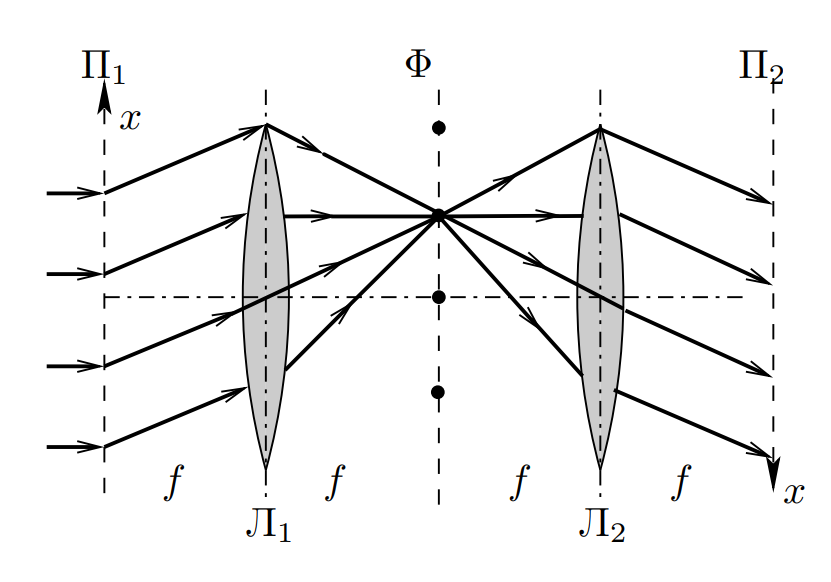
\includegraphics[width=0.8\linewidth]{Screenshot_1}
	\caption{Двойная дифракция Аббе}
	\label{fig:screenshot1}
\end{figure}


\parag{Пространственная фильтрация}

В фурье-плоскости возможно избирательное воздействие на разные пространственные гармоники: установив в любой точке $ x $ этой плоскости пластинку, вносящую определённое поглощение, мы изменим амплитуду и фазу плоской волны с пространственной частотой $ u = k x / f $, не изменяя амплитуд и фаз других плоских волн.

\parag{Мультипликация изображения}

Изображение, возникающее в плоскости $ П_2 $, представляет собой периодически повторяющееся с периодом $$ d_0 = \lambda f / d $$ изображение объекта с функцией пропускания $ f_0 (x) $.
Соседние элементы периодической структуры, видимой в $ П_2, $ $ f(x) = \Sigma f_0(x-n d_0) $, не налагаются друг на друга при условии $ d_0 > a $, где $ a $ -- размер объекта. Число элементов $ N $ размноженного изображения определяется шириной главного максимума картины дифракции Фраунгофера на отдельной щели решётки: $$ N\approx 2 b / d_0. $$

\parag{Разрешающая способность. Критерий Рэлея} 

Согласно качественному критерию, предложенному Рэлеем, два источника света различимы, если дифракционный максимум одного приходится на минимум другого. Т. е, расстояние между центрами пятен $ \Delta x $ равно полуширине пятна Эйри: 
\[\Delta x = 1.22 \frac{\lambda}{D} z,\] где $ z $ -- расстояние от диафрагмы до плоскости наблюдения, а $ D $ -- диаметр диафрагмы. Отсюда минимальное угловое разрешение равно: \[\alpha_{min} \approx 1.22 \frac{\lambda}{D}.\]

\parag{Расчётные формулы} ~\\

Минимально разрешаемое объективом расстояние:
\begin{equation}\label{минимальное_расстояние}
	l_{min}\approx \frac{2 f \lambda}{D},
\end{equation}
где $ f $ -- фокусное расстояние линзы.

Условия главных максимумов:
\begin{equation}\label{условие_максимумов}
	d \sin \theta_x = m_x \lambda, \;\;\;	d \sin \theta_y = m_y \lambda,
\end{equation}
где $ m_{x, y} $ -- порядок дифракционных максимумов.

Увеличение системы собирающих линз (в условиях опыта):
\begin{equation}\label{увеличение}
	\Gamma = \frac{b_1 b_2}{a_1 a_2},
\end{equation}
где $ a, \; b $ -- соответствующие расстояния на рис. \ref{fig:screenshot3}.

\begin{figure}[tbp]
	\centering
	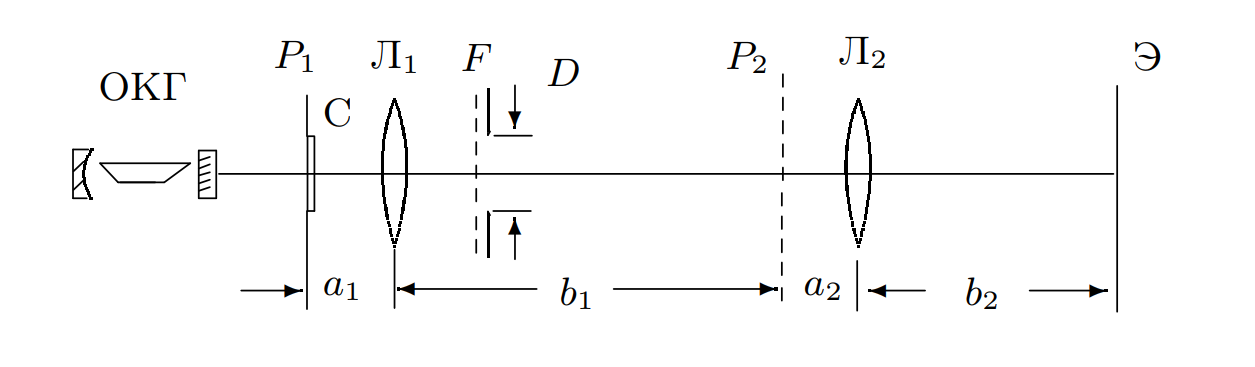
\includegraphics[width=0.8\linewidth]{Screenshot_3}
	\caption{Схема экспериментальной установки}
	\label{fig:screenshot3}
\end{figure}

\parag {Экспериментальная установка}~\\
Схема экспериментальной установки отображена на рис. \ref{fig:screenshot3}. Излучение лазера (ОКГ) почти перпендикулярно падает на сетку С, установленную вблизи фокальной плоскости линзы $ Л_1 $ — объектива. Вторичное изображение из плоскости $ P_2 $ проецируется на экран Э линзой $ Л_2 $.


Установка имеет следующие параметры:
\begin{enumerate}
    \item Длина волны лазера: $\lambda = 532 \; нм.$   
    \item Фокусное расстояние линзы $Л_1$: $f_1 = 110 \; мм.$
    \item Фокусное расстояние линзы $Л_2$: $f_2 = 25\; мм.$
\end{enumerate}

\parag {Ход работы} ~\\

\point Определение периодов решеток.

Расстояние от сетки до экрана: $H = 120 \; см.$ 
Из формул (\ref{условие_максимумов}), где $ \sin \theta \sim a / H $ и $ a $ -- период изображения, получим результат в табл. \ref{tabl:periods}.

\begin{table}[h]
\centering
\begin{tabular}{|c|c|c|}
\hline 
    Номер решетки & Период изображения, мм. & Период решетки, мм. \\ \hline
    1 & 30.0 & 0.0213 \\ \hline
    2 & 22.5 & 0.0284 \\ \hline
    3 & 12.0 & 0.0532 \\ \hline
    4 & 5.0 & 0.1277 \\ \hline
    5 & 3.7 & 0.1725 \\ \hline

\end{tabular}
\caption{Результаты вычислений периодов решеток по картине спектра}
\label{tabl:periods}
\end{table}

\point Соберем микроскоп со следующими параметрами. 

\[a_1 = 19      \; см,\]
\[b_1 = 48.7    \; см,\]
\[a_2 = 2.5     \; см,\]
\[b_2 = 77.5    \; см.\]

По формуле (\ref{увеличение}), $ \Gamma = 79.46$. Тогда найдём период решётки (табл. \ref{tabl:periods_microscope}).

\begin{table}[h]
\centering
\begin{tabular}{|c|c|c|}
\hline 
    Номер решетки & Период изображения, мм. & Период решетки, мм. \\ \hline
    1 & 1.0 & 0.0126 \\ \hline
    2 & 2.0 & 0.0252 \\ \hline
    3 & 3.3 & 0.0415 \\ \hline
    4 & 6.0 & 0.0755 \\ \hline
    5 & 9.0 & 0.1133 \\ \hline

\end{tabular}
\caption{Результаты вычислений периодов решеток по увеличенному изображению}
\label{tabl:periods_microscope}
\end{table}

\point Определим периоды решеток с помощью критерия Риэля.

Измерим наименьший размер диафрагмы, при котором еще видно изображение сетки. А далее по формуле (\ref{минимальное_расстояние}) определим периоды решоток. Результат занесем в таблицу \ref{tabl::periods_riel}.

\begin{table}[h]
\centering
\begin{tabular}{|c|c|c|}
\hline 
Номер решетки & Минимальный размер диафрагмы, мм. & Период решетки, мм. \\ \hline
1 & 4.0 & 0.0126 \\ \hline
2 & 4.0 & 0.0252 \\ \hline
3 & 2.5 & 0.0415 \\ \hline
4 & 1.6 & 0.0755 \\ \hline
5 & 1.1 & 0.1133 \\ \hline

\end{tabular}
\caption{Результаты вычислений периодов решеток по критерию Риэля}
\label{tabl:periods_riel}
\end{table}

\point Проверим метод Аббе.

Построим график $d = f(1 / D)$, где $d$ -- периоды решеток, расчитанные по спектрам, а $D$ -- минимальный размер диафрагмы.

\begin{figure}[h]
	\centering
	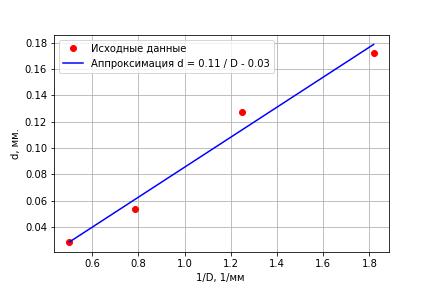
\includegraphics[width=0.8\linewidth]{abbe_graph.png}
	\caption{График зависимости $d(1/D)$}
	\label{fig:abbe_graph}
\end{figure}

Из графика получаем экспериментальный коэффициент: $k_{эксп} = 0.114$, в то время как теоретический: $k_{теор} = 2 \lambda f = 0.117$. Как видно, они хорошо совпадают, а значит метод Аббе работает верно.

\parag {Заключение} ~\\
В ходе работы мы определили несколькими способами периоды решёток, исследовали зависимость дифракционного предела разрешения объектива микроскопа от его диаметра. Отличия в полученных значениях периодов решоток могут быть связаны с общим недостатком метода, например, с точным определением фокусного расстояния: изображение может быть достаточно четким на довольно большом диапазоне расстояний и др.

\end{document}
